%
% File: chap01.tex
% Author: Zeller Quentin
% Description: Introduction
%
%\let\textcircled=\pgftextcircled
\chapter{OpenCV \& Flask}
\label{chap:OpenCV}

\initial{O}penCV est une librairie multiplate-forme \footnote{MacOS, IOS, Android, Windows, Linuxes,...} et open source pr�vue pour le machine learning ainsi que pour le traitement d'image (computer vision)\cite{opencv}. Du fait de sa licence BSD, cette librairie est constamment am�lior�e par le march� et notamment par les plus grosses entreprises du secteur technologique, ce qui en fait une des librairies leader dans ce domaine. En plus d'�tre disponible sur la quasi totalit� des syst�mes d'exploitations du march� elle est �galement disponible dans multiple langage que sont : C++, C, Python, Java and MATLAB � ce jour et sans compter �videmment les diff�rents binding. Nous utiliserons ici la librairie pour Python qui est un langage certes moins optimis� que certains de ses concurrents mais qui � l'instar de Mathlab permet de se concentrer sur le coeur du sujet. Il dispose en outre d'une bonne communaut� et d'un bon support.

Une autre particularit� d'OpenCV et ce qui le rend attractif � l'heure actuelle est sa compatibilit� avec les processeurs Nvidia et leurs CUDA \footnote{CUDA : Technologie dite GPGPU (General-Purpose Computing on Graphics Processing Units)} Core\cite{opencv_cuda}. Gr�ce aux avanc�es des GPUs a l'heure actuelle, principalement due au jeux vid�o mais aussi et principalement au crypto-monnaie les performances sont accrue d'un facteur 30x dans le pire des cas.



%=======
\section{Fonctionnement g�n�ral}
\label{sec:sec03a}
OPENCV

\section{Environnement de d�veloppement de l'application test}
\label{sec:sec03b}
pycharm opencv, livrairies, flask...

\definecolor{mygreen}{rgb}{0,0.6,0}
\definecolor{mygray}{rgb}{0.5,0.5,0.5}
\definecolor{mymauve}{rgb}{0.58,0,0.82}
\definecolor{deepred}{rgb}{0.6,0,0}

\lstset{
	language=Python,
	backgroundcolor=\color{white},   % choose the background color
	basicstyle=\footnotesize,        % size of fonts used for the code
	breaklines=true,                 % automatic line breaking only at whitespace
	captionpos=b,                    % sets the caption-position to bottom
	commentstyle=\color{mygreen},    % comment style
	escapeinside={\%*}{*)},          % if you want to add LaTeX within your code
	keywordstyle=\color{blue},       % keyword style
	emphstyle=\ttb\color{deepred},
	stringstyle=\color{mymauve},     % string literal style
}


	\lstinputlisting[language=Python, firstline=7, lastline=37, caption={Live streaming MJPEG with Flask, inspired from Miguel Grinberg. \cite{grinberg}}]{../../app/video_streaming_with_flask_example/main.py}
%	\caption{Live streaming MJPEG with Flask, inspired from Miguel Grinberg. \cite{grinberg}}





\begin{figure}[h]
	\centering
	\frame{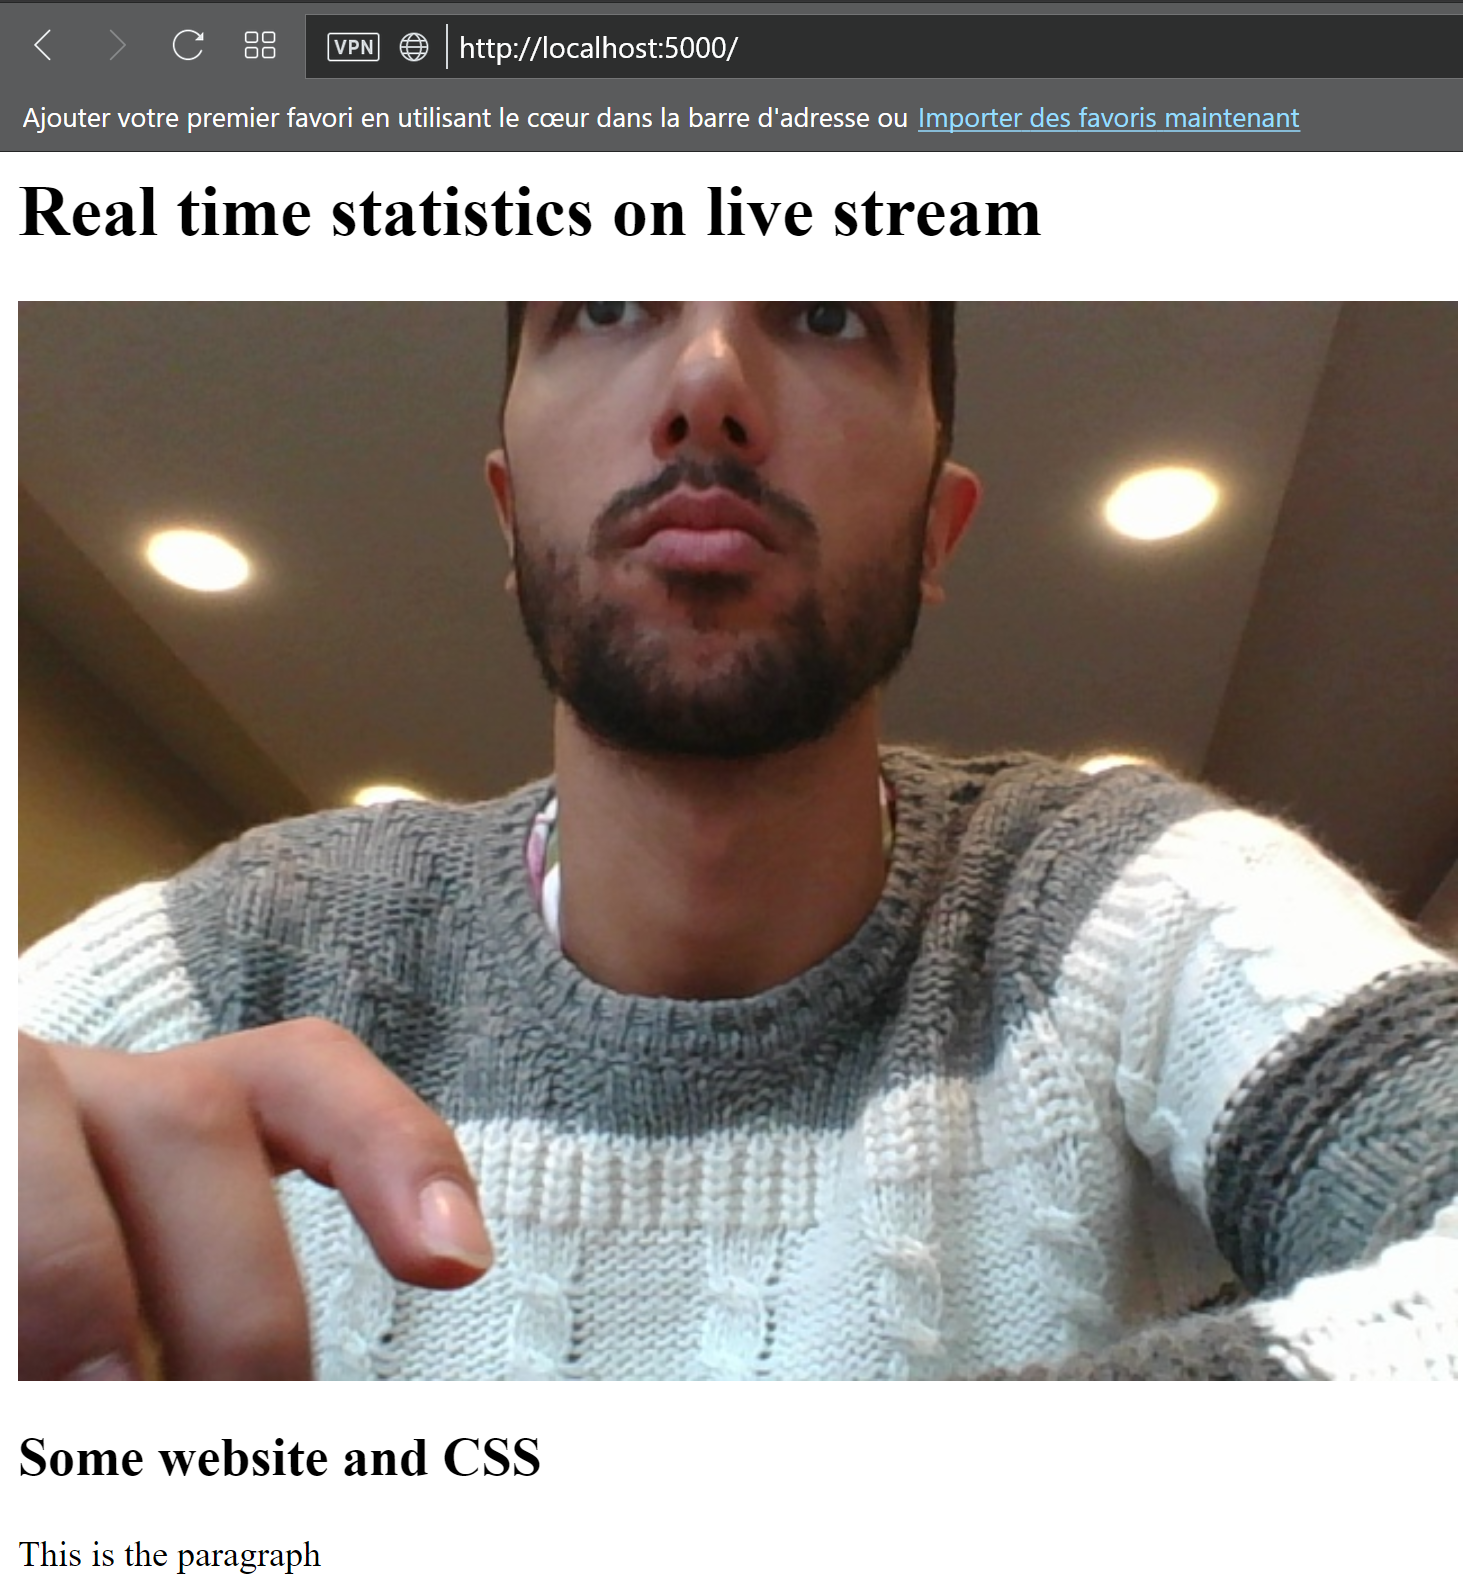
\includegraphics[width=0.8\linewidth]{fig01/website}}
	\mycaption[The easy Flask website MJPEG.]{Streaming HTTP avec librairie python Flask}
	\label{fig:flask}
	
\end{figure}

\begin{figure}[h]
	\centering
	\frame{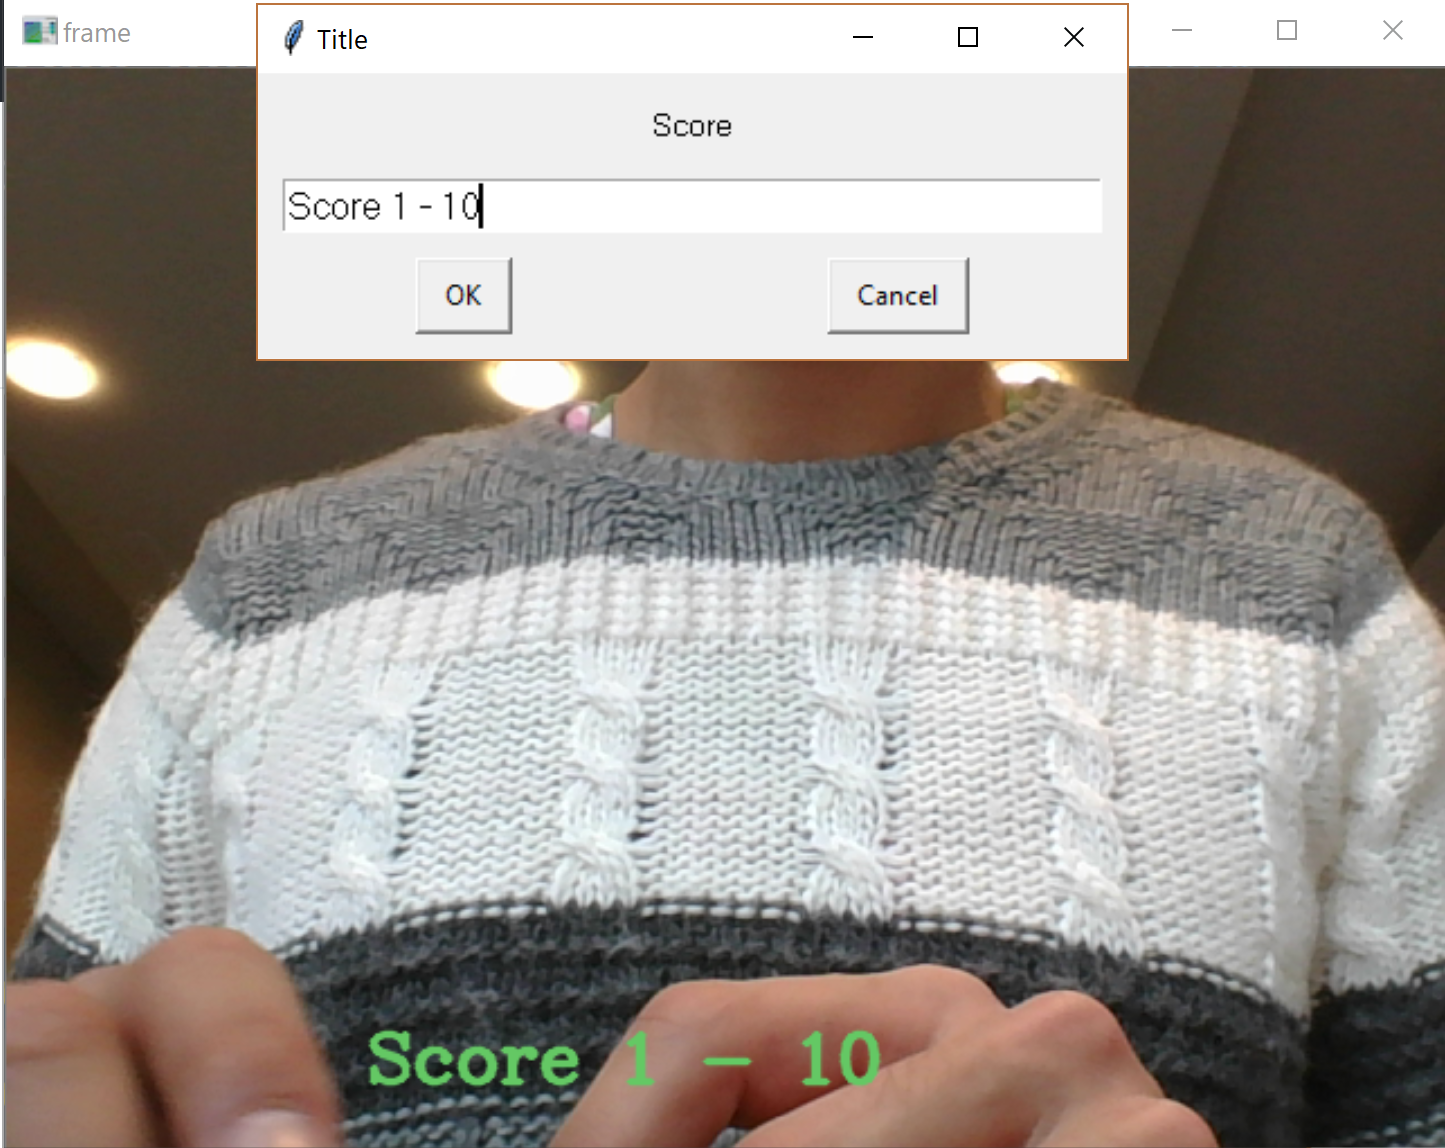
\includegraphics[width=0.8\linewidth]{fig01/example_application}}
	\mycaption[Burn text on live stream, display on GUI]{Int�gration texte dans vid�o live, affichage GUI bureau}
	\label{fig:live_text_integration}
	
\end{figure}

\begin{figure}[h]
	\centering
	\frame{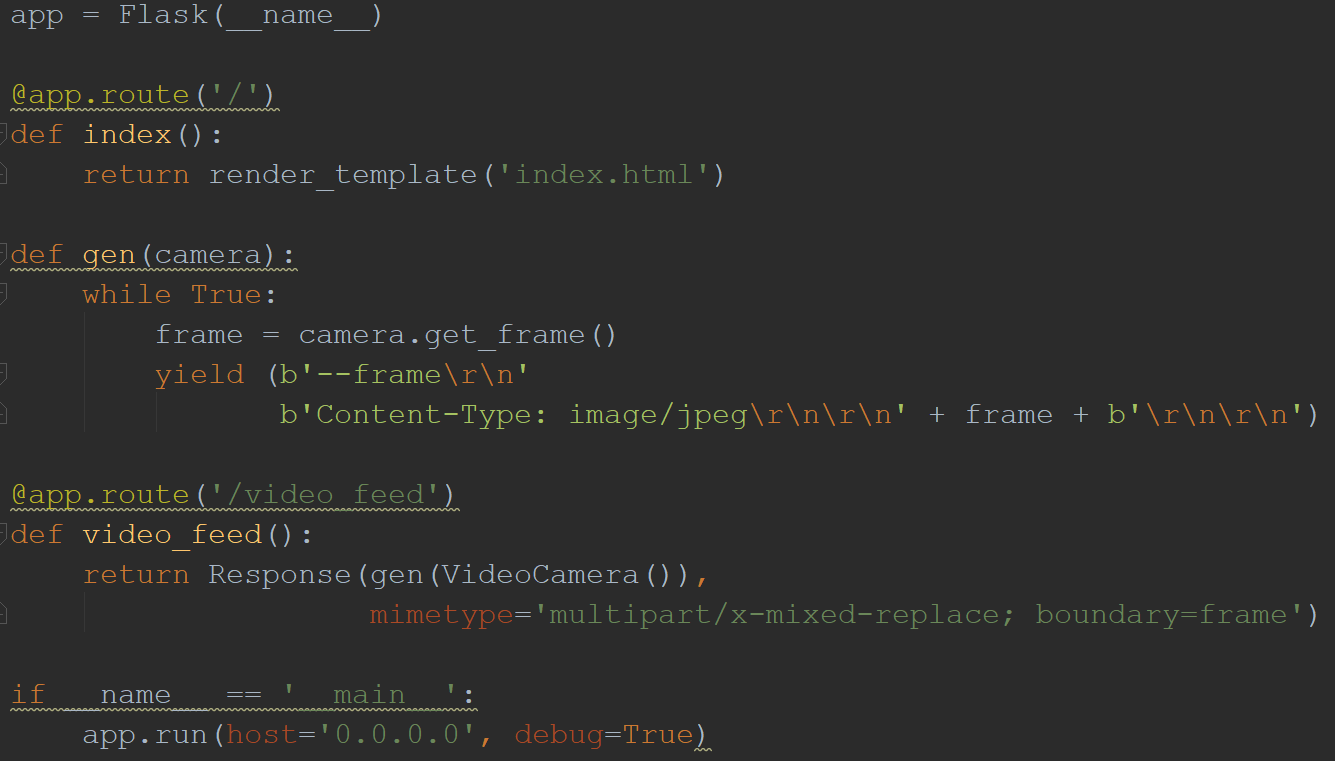
\includegraphics[width=1\linewidth]{fig01/flask_simple}}
	\mycaption[The easy Flask website MJPEG. (code)]{Code pour streaming HTTP avec librairie python Flask}
	\label{fig:flask_code}
	
\end{figure}


\section{Environnement de production}
\label{sec:sec03c}
\subsection{The Opera hybrid TV option}
\label{subsec:subsec03c}


%=========================================================